% !TEX TS-program = XeLaTeX
% !TEX spellcheck = en-US
\documentclass[aspectratio=169]{beamer}

\usetheme{example}

\usepackage{tikz}
\usetikzlibrary{positioning, arrows.meta, calc}

\title{Lecture 9:\\ Neural networks}
\institute{GRA4160: Predictive modelling with machine learning}
\date{March 4th 2026}
\author{Vegard H\o ghaug Larsen}

\begin{document}

\maketitle

\frame{
	\frametitle{Plan for today:}
	\begin{itemize}
		\item Introduction to neural networks
		\item Single layer (feed forward) neural networks
		\item Fitting a Neural Network
		%\item Backpropagation
		%\item Stochastic gradient descent
	\end{itemize}}

\frame{
	\frametitle{Introduction to neural networks}
	\begin{itemize}
		\item A neural network is a computational system that is inspired by the structure and function of the human brain
		      \pause
		\item It consists of many interconnected processing units, called neurons, that work together to solve complex problems
		      \pause
		\item Each neuron receives input from other neurons, processes that input, and then produces an output that is sent to other neurons
		      \pause
		\item By combining and processing information in this way, a neural network can learn to recognize patterns and make predictions
	\end{itemize}
}

\frame{
	\frametitle{Single layer (feed forward) neural networks}

	\begin{itemize}
		\item A single layer neural network is a model that takes a set of $p$ input variables $X=(X_1,X_2,...,X_p)$
		      \pause
		\item The NN is a nonlinear function $f(X)$ that maps the input variables to an output variable $Y$
		      \pause
		\item The weights $w_1,w_2,...,w_p$ are the parameters of the model, controlling the strength of the relationship between the input variables and the output variable
		      \pause
		\item Given a nonlinear activation function $g(z)$, the model can be written as a sum of $K$ activation functions
	\end{itemize}
	\[ Y = f(X) = \beta_0 + \sum_{k=1}^K\beta_k g\left(w_{k0} + \sum_{j=1}^pw_{kj}X_j\right) \]
}

\frame{
\frametitle{Neural network with a single hidden layer}
\centering
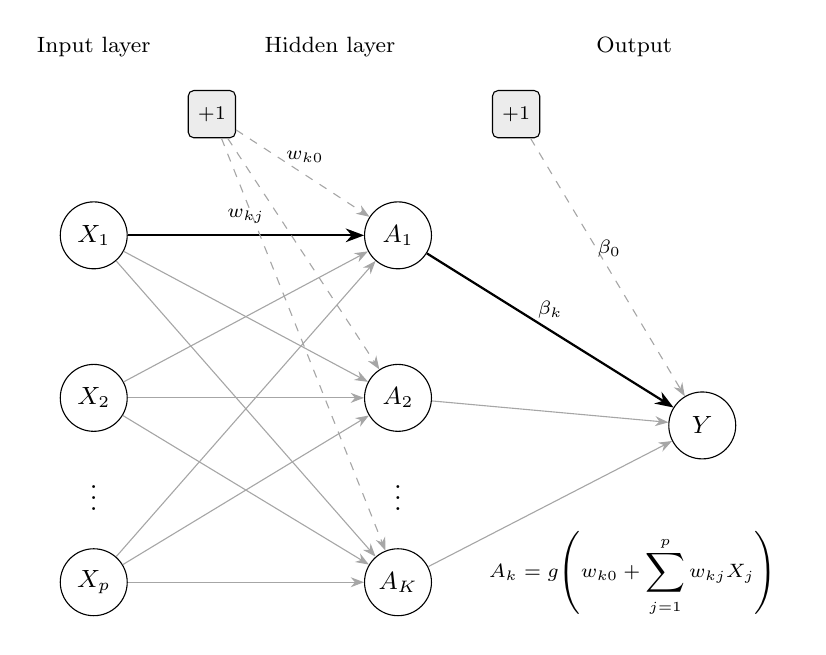
\begin{tikzpicture}[
	node distance=1.2cm and 3cm,
	neuron/.style={circle, draw, minimum size=0.85cm, inner sep=0pt, font=\small},
	bias/.style={rectangle, draw, rounded corners=2pt, minimum size=0.6cm, inner sep=2pt, font=\scriptsize, fill=gray!15},
	>=Stealth,
]
	% Input layer
	\node[neuron] (x1) {$X_1$};
	\node[neuron, below=of x1] (x2) {$X_2$};
	\node[below=0.35cm of x2] (xdots) {$\vdots$};
	\node[neuron, below=0.35cm of xdots] (xp) {$X_p$};

	% Bias node for hidden layer
	\node[bias, above=0.8cm of x1, xshift=1.5cm] (b1) {$+1$};

	% Hidden layer
	\node[neuron, right=of x1] (h1) {$A_1$};
	\node[neuron, below=of h1] (h2) {$A_2$};
	\node[below=0.35cm of h2] (hdots) {$\vdots$};
	\node[neuron, below=0.35cm of hdots] (hK) {$A_K$};

	% Bias node for output layer
	\node[bias, above=0.8cm of h1, xshift=1.5cm] (b2) {$+1$};

	% Output layer
	\node[neuron, right=of h2, yshift=-0.35cm] (y) {$Y$};

	% Connections: input -> hidden (gray, thin)
	\foreach \i in {x1, x2, xp} {
		\foreach \h in {h1, h2, hK} {
			\draw[->, gray!70] (\i) -- (\h);
		}
	}

	% Highlight one connection for weight label
	\draw[->, thick] (x1) -- (h1);

	% Connections: bias -> hidden
	\foreach \h in {h1, h2, hK} {
		\draw[->, dashed, gray!70] (b1) -- (\h);
	}

	% Connections: hidden -> output (gray, thin)
	\foreach \h in {h1, h2, hK} {
		\draw[->, gray!70] (\h) -- (y);
	}

	% Highlight one connection for beta label
	\draw[->, thick] (h1) -- (y);

	% Connections: bias -> output
	\draw[->, dashed, gray!70] (b2) -- (y);

	% Layer labels
	\node[above=0.3cm of b1, xshift=-1.5cm, font=\footnotesize] {Input layer};
	\node[above=0.3cm of b1, xshift=1.5cm, font=\footnotesize] {Hidden layer};
	\node[above=0.3cm of b2, xshift=1.5cm, font=\footnotesize] {Output};

	% Weight labels
	\node[font=\scriptsize, above=1pt] at ($(x1)!0.5!(h1)$) {$w_{kj}$};
	\node[font=\scriptsize, above=1pt] at ($(h1)!0.5!(y)$) {$\beta_k$};

	% Bias labels
	\node[font=\scriptsize, above=1pt] at ($(b1)!0.5!(h1)$) {$w_{k0}$};
	\node[font=\scriptsize, above=1pt] at ($(b2)!0.5!(y)$) {$\beta_0$};

	% Formula annotations next to hidden nodes
	\node[font=\scriptsize, right=0.6cm of hK, yshift=0.1cm, text width=3.8cm, align=left] {$A_k = g\!\left(w_{k0} + \displaystyle\sum_{j=1}^p w_{kj}X_j\right)$};
\end{tikzpicture}
}

\frame{
	\frametitle{Hidden units and the output layer}
	The network is built up in two steps:
	\begin{enumerate}
		\item Specify the number of hidden units $K$ and the activation function $g(X)$ and we can calculate $K$ activations in the hidden layer as
		      \[A_k = h_k(X) = g\left(w_{k0} + \sum_{j=1}^pw_{kj}X_j\right) \]
		      \pause
		\item The $K$ activations feed into the output layer, which is a linear function of the activations
		      \[ f(X) = \beta_0 + \sum_{k=1}^K\beta_k A_k \]
	\end{enumerate}
}

\frame{
	\frametitle{The forward pass as matrix multiplications}
	We can write the forward pass compactly using matrices. Let $\mathbf{X}$ be the $n \times p$ input matrix and define:
	\pause
	\begin{enumerate}
		\item \textbf{Hidden layer:} Compute the $n \times K$ matrix of activations
		      \[ A_{ik} = g\!\left(w_{k0} + \sum_{j=1}^p w_{kj}X_{ij}\right) \quad\Longleftrightarrow\quad \mathbf{A} = g\!\left(\mathbf{1}_{n}\mathbf{w}_0^\top + \mathbf{X}\mathbf{W}^\top\right) \]
		      where $\mathbf{W}$ is the $K \times p$ weight matrix, $\mathbf{w}_0$ is the $K \times 1$ bias vector, and $g(\cdot)$ is applied element-wise
		      \pause
		\item \textbf{Output layer:} Compute the $n \times 1$ output vector
		      \[ Y_i = \beta_0 + \sum_{k=1}^K \beta_k A_{ik} \quad\Longleftrightarrow\quad \mathbf{Y} = \beta_0\mathbf{1}_{n} + \mathbf{A}\boldsymbol{\beta} \]
		      where $\boldsymbol{\beta} = (\beta_1,\ldots,\beta_K)^\top$
	\end{enumerate}
	\pause
	\smallskip
	Each layer is a matrix multiplication followed by an activation function --- this is what makes neural networks efficient to compute on GPUs
}

\frame{
	\frametitle{What does the activation function look like?}
	Activation functions are used to introduce non-linearity and enable the network to learn complex patterns in the input data. Here are some common activation functions used in neural networks:
	\begin{enumerate}
		\item The sigmoid function (we also used this for logistic regression)
		      \[ g(z) = \frac{1}{1+e^{-z}} \]
		      \pause
		\item Rectified Linear Unit (ReLU)
		      \[ g(z) = \max(0, z) \]
		      \pause
		\item Softmax (typically used in the output layer for multi-class classification)
		      \[ g(z_i) = \frac{\exp(z_i)}{\sum_{j=1}^{K} \exp(z_j)} \]
	\end{enumerate}
}

\frame{
\frametitle{Sigmoid vs ReLU}
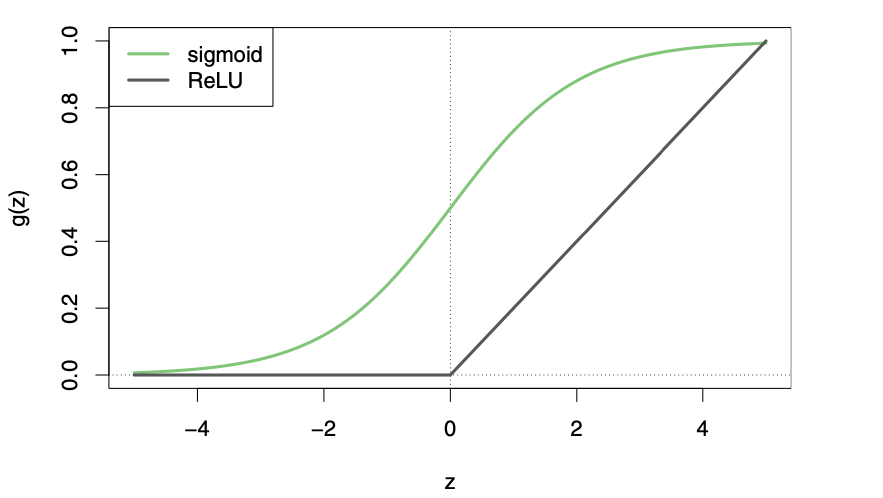
\includegraphics[scale=0.35]{figures/sigmoid_vs_relu.png}\\
{\footnotesize Source: An Introduction to Statistical Learning, James, Witten, Hastie and Tibshirani, 2021}
}


\frame{
	\frametitle{Fitting a Neural Network}
	We can fit the parameters of a neural network by minimizing a cost function (nonlinear least squares)

	\[ \min_{w_k,\beta} \frac{1}{2}\sum_{i=1}^n \left( y_i - f(x_i) \right)^2 \]

	where

	\[ f(X) = \beta_0 + \sum_{k=1}^K\beta_k g\left(w_{k0} + \sum_{j=1}^p w_{kj}X_j\right) \]

	\pause

	This is a nonlinear optimization problem, and it is not straightforward to solve.
}

\frame{
	\frametitle{Gradient descent}
	We can use gradient descent to find the optimal parameters. Let's put all the parameters in one vector $\theta$ and define the cost function as

	\[ L(\theta) = \frac{1}{2}\sum_{i=1}^n \left( y_i - f_\theta(x_i) \right)^2 \]

	\pause
	Then, to find the optimal parameters, we can use gradient descent to minimize the cost function $L(\theta)$ by the following iterative update rule:
	\begin{enumerate}
		\item Let $\theta^t$ be a vector of all the parameters in the system at iteration $t$. Start with an initial guess $\theta^0$
		      \pause
		\item Update the parameters according to the following rule: $\theta^{t+1} = \theta^t + \delta$, where $\delta$ is a vector that reflects a small change in the parameters such that
		      \[ L(\theta^{t+1})<L(\theta^{t}) \]
		\item Repeat until convergence
	\end{enumerate}
}

\frame{
\frametitle{How do we know how to update the parameters (what is $\delta$)?}

We need to calculate the gradient of the cost function $L(\theta)$ with respect to the parameters $\theta$:

\[ \nabla L(\theta^t) = \left.\frac{\partial L(\theta)}{\partial \theta}\right|_{\theta=\theta^t} = \left.\frac{\partial}{\partial \theta} \frac{1}{2}\sum_{i=1}^n \left( y_i - f_\theta(x_i) \right)^2\right|_{\theta=\theta^t} \]

\pause
$\nabla L(\theta^t)$ gives us the directions to move $\theta$ so as to decrease the objective $L(\theta)$\\
\pause
\smallskip
Given a learning rate $\eta$, we can use the gradient to update the parameters as follows:
\[ \theta^{t+1} = \theta^t - \eta \nabla L(\theta^t) \]
\pause
The gradient packs all the partial derivatives into a single vector: $\nabla L = \left[ \frac{\partial L}{\partial \beta_k}, \frac{\partial L}{\partial w_{kj}} \right]^T$
}

\frame{
	\frametitle{Backpropagation: setup}
	Recall the forward pass for observation $i$. Define the intermediate quantities:
	\begin{align*}
		z_{ik}    & = w_{k0} + \sum_{j=1}^p w_{kj}\, x_{ij}            & & \text{(pre-activation for hidden unit } k\text{)} \\
		A_{ik}    & = g(z_{ik})                                          & & \text{(activation for hidden unit } k\text{)}     \\
		f_i       & = \beta_0 + \sum_{k=1}^K \beta_k\, A_{ik}           & & \text{(network output)}                            \\
		L_i       & = \tfrac{1}{2}\left( y_i - f_i \right)^2            & & \text{(loss for observation } i\text{)}
	\end{align*}
	\pause
	The total loss is $L(\theta) = \sum_{i=1}^n L_i$. We need $\frac{\partial L_i}{\partial \beta_k}$ and $\frac{\partial L_i}{\partial w_{kj}}$.\\
	\smallskip
	The key idea: apply the \textbf{chain rule} layer by layer, working \emph{backwards} from the loss to the parameters.
}

\frame{
	\frametitle{Backpropagation: the chain rule}
	\textbf{Step 1:} The common starting point --- derivative of the loss w.r.t.\ the output:
	\[ \frac{\partial L_i}{\partial f_i} = -(y_i - f_i) \]
	\pause
	\textbf{Step 2:} Derivative w.r.t.\ the output-layer weights $\beta_k$ (one link in the chain):
	\[ \frac{\partial L_i}{\partial \beta_k} = \underbrace{\frac{\partial L_i}{\partial f_i}}_{-(y_i - f_i)} \cdot \underbrace{\frac{\partial f_i}{\partial \beta_k}}_{A_{ik}} = -(y_i - f_i)\cdot A_{ik} \]
	\pause
	\textbf{Step 3:} Derivative w.r.t.\ the hidden-layer weights $w_{kj}$ (three links in the chain):
	\[ \frac{\partial L_i}{\partial w_{kj}} = \underbrace{\frac{\partial L_i}{\partial f_i}}_{-(y_i - f_i)} \cdot \underbrace{\frac{\partial f_i}{\partial A_{ik}}}_{\beta_k} \cdot \underbrace{\frac{\partial A_{ik}}{\partial z_{ik}}}_{g'(z_{ik})} \cdot \underbrace{\frac{\partial z_{ik}}{\partial w_{kj}}}_{x_{ij}} = -(y_i - f_i)\cdot\beta_k\cdot g'(z_{ik})\cdot x_{ij} \]
	\pause
	\smallskip
	Each parameter receives a fraction of the residual $(y_i - f_i)$ propagated \emph{back} through the network --- hence the name \textbf{backpropagation}.
}

\frame{
	\frametitle{Stochastic gradient descent (SGD)}
	\begin{itemize}
		\item SGD is a method for minimizing a cost function by iteratively moving in the direction of steepest descent as defined by the negative of the gradient
		      \pause
		\item In contrast to batch gradient descent, which computes the gradient of the cost function over the entire dataset, SGD computes the gradient on a single training example at a time
		      \pause
		\item This makes SGD much faster than batch gradient descent, but it also means that SGD is much noisier
		      \pause
		\item The noise can be reduced by averaging the gradients over several training examples
	\end{itemize}
}

\frame{
	\frametitle{L2 regularization}
	\begin{itemize}
		\item L2 regularization adds a penalty term to the cost function to prevent overfitting
		\item The penalty term is proportional to the sum of the squares of the weights in the network
		\item The regularized cost function is
	\end{itemize}
	\[ L_{\text{reg}}(\theta) = \frac{1}{2}\sum_{i=1}^n \left( y_i - f_\theta(x_i) \right)^2 + \lambda \sum_{k,j} w_{kj}^2 \]
	where $\lambda$ is the regularization parameter controlling the trade-off between fit and complexity
}

\frame{
	\frametitle{Dropout}
	\begin{itemize}
		\item Dropout is a regularization technique that randomly drops out (sets to zero) some of the neurons in the network during training
		\item This helps prevent the network from overfitting to the training data
		\item Dropout can be seen as an ensemble of all the networks that can be formed by dropping out different neurons
		\item Typical dropout rates are between 0.2 and 0.5, and dropout is only applied during training, not at inference time
	\end{itemize}
}
\end{document}
